\documentclass[11pt]{scrartcl}
\usepackage[utf8]{inputenc}
\usepackage[sexy]{evanchen} 
\usepackage{graphicx}
\graphicspath{{8 Outsource K Math/Gambar/}}

\title{Segitiga}
\author{Azzam and Akeyla}
\date{Maret 2023}

\begin{document}

\maketitle

\renewcommand*\contentsname{Daftar Isi}
\tableofcontents

\newpage

\section{Angle Chasing}
\subsection{Definisi}
Angle Chasing merupakan sebuah teknik yang digunakan untuk mencari properti dari sebuah konfigurasi geometri dengan menghitung besar sudut yang ada. Perhitungan besar sudut ini bisa menggunakan berbagai properti yang tersedia.
\subsection{Beberapa properti sudut yang bisa diperhatikan}
\begin{enumerate}
    \item Segitiga ABC merupakan segitiga sama kaki dengan $AB=AC$ jika dan hanya jika $\angle{ABC}=\angle{ACB}$.
    \item Sebuah segitiga merupakan segitiga sama sisi jika dan hanya jika seluruh sudutnya memiliki besar $60^{\circ}$.
    \item Apabila sebuah segitiga merupakan segitiga siku-siku, maka besar sudutnya pasti dalam bentuk $90^{\circ}, \theta, 90^{\circ} - \theta$.
    \item Apabila sebuah segitiga memiliki panjang sisi dengan rasio $1:\sqrt{3}:2$ maka besar sudutnya secara berurutan adalah $30^{\circ},60^{\circ},90^{\circ}$.
    \item Jumlah sudut di segi-$n$ adalah $(n-2)\times 180^{\circ}$.
    \item \begin{figure}[h]
        \centering
        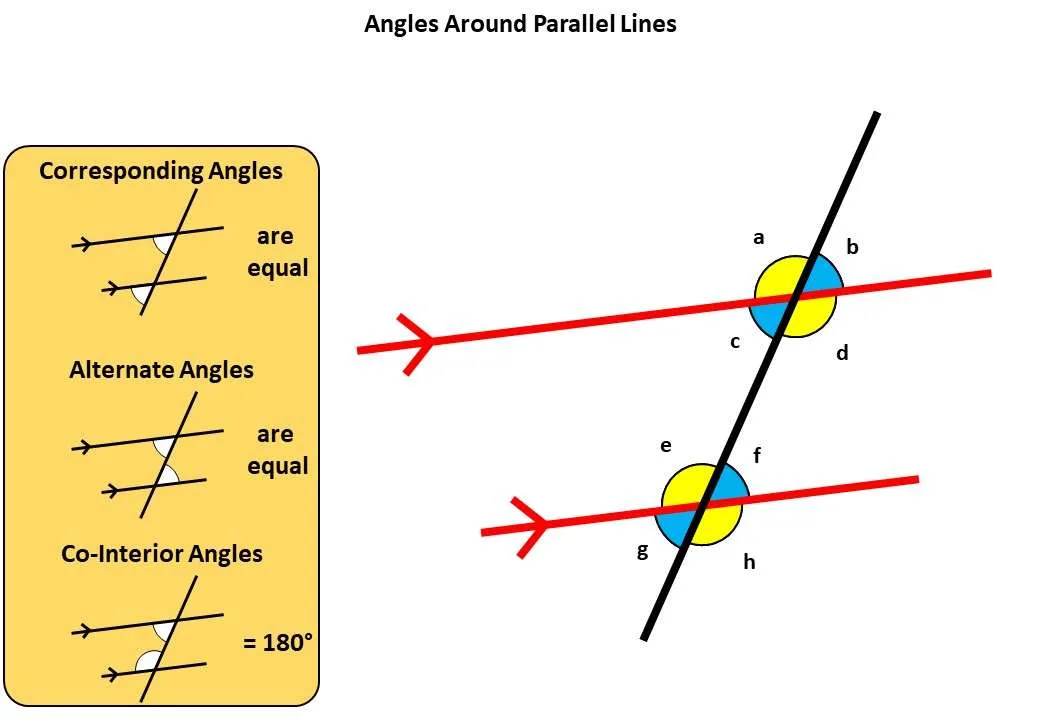
\includegraphics[width=0.7\textwidth]{Parallel.png}
        \label{fig:my_label}
    \end{figure}
\end{enumerate}

\section{Lingkaran}
\subsection{Definisi}
\begin{enumerate}
    \item Sudut pusat adalah sudut yang diapit oleh dua jari-jari lingkaran. Sudut ini terbentuk dari tiga titik. Dua titik di antaranya merupakan titik di keliling lingkaran dan satu titik lainnya adalah titik pusat lingkaran.
    \item Sudut keliling adalah sudut yang terbentuk dari tiga titik di keliling lingkaran. Sudut ini dibatasi oleh dua tali busur.
    \item Sudut keliling $ACB$ dan sudut pusat $AOB$ keduanya menghadap busur yang sama, $AB$.
    \item Dua sudut keliling disebut berlawanan apabila kedua sudut keliling tersebut menghadap tali busur yang sama tetapi busurnya berbeda
    \item Garis $\ell$ disebtu menyinggung lingkaran $\omega$ apabila garis $\ell$ melewati tepat satu titik di keliling lingkaran $\omega$
\end{enumerate}

\subsection{Properti sudut pada lingkaran}
\begin{enumerate}
    \item Sebuah sudut keliling akan memiliki besar setengah dari sudut pusat yang menghadap busur yang sama
    \item Dua sudut keliling yang menghadap busur yang sama akan memiliki besar yang sama
    \item Dua sudut keliling yang menghadap busur yang memiliki panjang sama akan memiliki besar yang sama
    \item Dua sudut keliling yang berlawanan memiliki jumlah sudut $180^{\circ}$
    \item Jika garis $\ell$ menyinggung lingkaran $\omega$ di titik $P$ dan $O$ adalah titik pusat lingkaran $\omega$ maka $OP$ akan tegak lurus dengan $\ell$
\end{enumerate}

\section{Latihan Komprehensif}
\begin{problem}
    \begin{figure}[h]
        \centering
        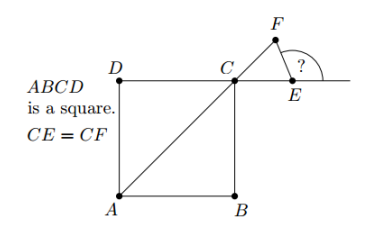
\includegraphics{AngleChasing.png}
        \label{fig:my_label}
    \end{figure}
\end{problem}

\begin{problem}
    (AHSME 1957) Diberikan sebuah segitiga $ABC$ dengan $BC > AC$. Titik $D$ terletak di $BC$ sedemikian hingga $CD = CA$. Apabila diketahui bahwa $\angle{CAB} - \angle{ABC} = 30^{\circ}$, besar sudut $\angle{BAD}$ adalah ...
\end{problem}

\begin{problem}
    (AMC 10B 2009) Sembilan buah trapesium sama kaki identik disusun menjadi seperti pada gambar berikut. Besar sudut terbesar yang ada di trapesium tersebut adalah ...
    \begin{figure}[h]
        \centering
        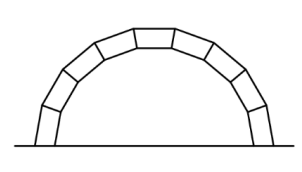
\includegraphics{Arch.png}
        \label{fig:my_label}
    \end{figure}
\end{problem}

\begin{problem}
    (Auckland MO Junior 2015) Garis bagi dalam dari sudut $A$ di jajargenjang $ABCD$ memotong sisi $BC$ di titik $M$. Diketahui bahwa garis bagi dalam sudut $AMC$ melewati titik $D$. Tentukan besar sudut $A$ apabila diketahui bahwa $\angle MDC = 45^{\circ}$.
    \begin{figure}[h]
        \centering
        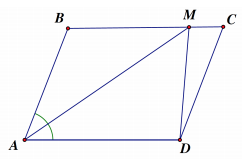
\includegraphics[width=0.5\linewidth]{AucklandMO2015PJ4.png}
    \end{figure}
\end{problem}

\begin{problem}
    (Afrika Selatan MO 2014) Diberikan segitiga tumpul $ABC$ yang tumpul di titik $A$. Titik $D, E, F$ secara berturut-turut adalah proyeksi titik $A, B, C$ ke sisi di hadapannya. Diketahui bahwa $DE$ sejajar dengan $CF$ dan $DF$ sejajar dengan garis bagi dalam $\angle BAC$. Tentukan besar semua sudut di segitiga tersebut.
\end{problem}

\begin{problem}
    (Auckland MO Junior 2019) Diberikan sebuah segiempat konveks $ABCD$ yang memenuhi $\angle BAC = 20^{\circ}$, $\angle CAD = 60^{\circ}$, $\angle ADB = 50^{\circ}$ , dan $\angle BDC = 10^{\circ}$. Tentukan besar sudut $\angle ACB$.
\end{problem}

\begin{problem}
    (Auckland MO Senior 2017) Garis tinggi segitiga $ABC$ berpotongan di titik $H$. Tentukan besar sudut $\angle ACB$ apabila diketahui $AB = CH$.
\end{problem}

\begin{problem}
    (Afrika Selatan MO 2015) Titik $E$ dan $F$ terletak di dalam persegi $ABCD$ sehingga $ABF$ dan $BCE$ merupakan segitiga sama sisi. Tentukan besar sudut $\angle EDF$.
\end{problem}

\end{document}